\documentclass[11pt, a4paper]{article}
\usepackage[left=2cm,right=2cm,top=2cm,bottom=2cm]{geometry}
\usepackage[utf8]{inputenc}
\usepackage[T1]{fontenc}
\usepackage{graphicx}
\usepackage[french]{babel}
\usepackage{fancyhdr}
\usepackage{fancyvrb}
\usepackage[hyphens]{url}
\usepackage{enumitem}
\usepackage{listings}
\usepackage{ulem}
\usepackage{spverbatim}

\newcommand\tab{\hspace*{12.5mm}}
\setlength\parindent{0pt}

\title{ \uline{\Huge{\textbf{Projet entrepôt de données}}} \\ Seattle Airbnb Open Data}
\author{Boursier Louis, Filaudeau Eloi, Lasherme Loïc, Nantier Matthias}
\date{}

\lstset{
   language=SQL,
   extendedchars=true,
   basicstyle=\scriptsize,
   literate=%
   {é}{{\'e}}{1}%
   {è}{{\`e}}{1}%
   {ê}{{\^e}}{1}%
   {à}{{\`a}}{1}%
}

\begin{document}

\maketitle
\vfill

\begin{center}
\url{https://github.com/loutouk/AirBnbDataWareHouse?fbclid=IwAR2pvwhMl38kLbcfEZWgI1Re0pcp3exHfyEBntjkolrTxXu8RAZyu1OxdeM}
\end{center}
\newpage
\tableofcontents
\newpage

\section{Introduction}
\tab Le but de ce projet était l'intégration de données dans un entrepôt de données. Pour cela nous devions trouver un exemple concret qui se rapproche de la réalité. Nous avons donc optés pour un exemple qui est : "les Airbnb de Seattle". Notre jeu de données provient du site web Kaggle qui est fournit directement par Airbnb sous une une licence CC0: Public Domain.
\vspace{5mm}

\begin{minipage}[t]{0.45\linewidth}
   \textbf{\Large{Contenu :}}
   \begin{itemize}[label=\textbullet]
      \item Les logements avec leurs propriétaires.
      \item Les avis des utilisateurs sur leurs résevrations.
      \item Les calendriers, c'est à dire les dates associées aux réservations à un certain prix, et leur disponibilité à cette date.
   \end{itemize}
\end{minipage}
\hfill
\begin{minipage}[t]{0.45\linewidth}
   \textbf{\Large{Idées :}}
   \begin{itemize}[label=\textbullet]
      \item Décrire les caractéristiques de chaque quartier de Seattle en utilisant la description des logements.
      \item Quelles sont les plus forts moments d'affluence ? Comment les prix varient ?
      \item Quelle est la tendance vis à vis des visiteurs à Seattle et des logements proposés ?
   \end{itemize}
\end{minipage}
\vspace{5mm}

Après avoir trouvé nos données, il a fallut les transformer, les nettoyer pour enfin faire nos requêtes dessus. Nous avons donc opté pour un schéma en étoile et de travailler avec MySQL 5.7, car impossible de travailler sous Oracle chez nous, \url{https://livesql.oracle.com/} est beaucoup trop lent, ne peut pas faire l'importation de fichier supérieur à 1Mb, et les sessions ont une durée limitée dans le temps.

\section{Conception de l'entrepôt}
\tab Pour créer notre entrepôt avec le jeu de données, nous avons dû réaliser plusieurs opérations. La première consistait à décomposer le jeu en plusieurs table afin de créer notre schéma en étoile. Ensuite nous avons dû nettoyer plusieurs fois les données, ce qui n'était pas chose aisée.

\subsection{Transformation des données}
\begin{enumerate}
   \item Créer une dimension date
   \begin{enumerate}[label=\roman*.]
      \item Créer un nouveau projet OpenRefine à partir du fichier \spverb"calendar.csv". Pour accélérer la vitesse des opérations, on peut ne charger qu'une partie des données \spverb"Load at most 100000 row(s) of data"
      \item Sous OpenRefine, créer une nouvelle colonne \spverb"year" depuis la colonne \spverb"date". \spverb|Edit column > Add column based on this colulmn > split(value, "-")[0]|
      \item Faire la même chose pour les mois et les jours
      \item Créer la clé dateId pour notre nouvelle table à partir de la colonne \spverb"calendar". Sa valeur est optenue avec l'expression suivante : \\ \spverb|sha1(cells.year.value+cells.month.value+cells.day.value).substring(0,10)|
      \item Supprimer les colonnes \spverb"date, available, price, listing_id" qui ne sont plus utiles \spverb|Edit column > Remove this column|
      \item Pour chaque table des dimensions, on enlève les duplicats, c'est à dire que chaque ligne doit être unique (2FN). Voir l'annexe \spverb"Removing duplicates" plus bas
      \item On peut maintenant exporter ce projet en csv, pour récupérer notre dimension date
   \end{enumerate}
   \item Créer une dimension localisation
   \begin{enumerate}[label=\roman*.]
      \item Créer un nouveau projet OpenRefine à partir du fichier \spverb"listings.csv"
      \item Ne garder que les colonnes \spverb"neighbourhood_cleansed, neighbourhood_group_cleansed" et \spverb"zipcode"
      \item Créer la clé localisationId pour notre nouvelle table à partir de nos trois colonnes. Sa valeur est optenue avec l'expression suivante : \spverb|sha1(value + row.cells.zipcode.value + row.cells.neighbourhood_group_cleansed.value).substring(0,10)|
      \item Comme avant, éliminer les duplicats
      \item Exporter ce projet en csv pour récupérer la dimension localisation
   \end{enumerate}
   \item Créer une dimension propriétaire
   \begin{enumerate}[label=\roman*.]
      \item Créer un nouveau projet OpenRefine à partir du fichier \spverb"listings.csv"
      \item Ne garder que les colonnes \spverb"host_id, host_name, host_since, host_response_time,"\\ \spverb"host_response_rate," \spverb"host_acceptance_rate, host_is_superhost"
      \item Renommer la clé \spverb"host_id" en \spverb"proprietaireId"
      \item Comme avant, éliminer les duplicats sur \spverb"proprietaireId"
      \item Exporter ce projet en csv pour récupérer la dimension propriétaire
   \end{enumerate}
   \item Créer une dimension logement
   \begin{enumerate}[label=\roman*.]
      \item Créer un nouveau projet OpenRefine à partir du fichier \spverb"listings.csv"
      \item Ne garder que les colonnes \spverb"name, summary, space, description"
      \item réer la clé \spverb"logementId" pour notre nouvelle table à partir de la colonne \spverb"name". Sa valeur est optenue avec l'expression suivante : \spverb|sha1(value).substring(0,10)|
      \item Comme avant, éliminer les duplicats sur \spverb|logementId|
      \item Exporter ce projet en csv pour récupérer la dimension logement
   \end{enumerate}
   \item Créer la première partie de la table des faits
   \begin{enumerate}[label=\roman*.]
      \item Créer un nouveau projet OpenRefine à partir du fichier \spverb|listings.csv|
      \item Ne garder que les colonnes \spverb|id, host_id, name, neighbourhood_cleansed,|\\ \spverb|neighbourhood_group_cleansed| et \spverb|zipcode|
      \item Recréer les colonnes correspondant aux clés des tables des dimensions à partir des colonnes gardées, comme fait dans les étapes précédentes
      \item Supprimer les colonnes gardées pour ne laisser que les colonnes générées correspondants aux clés des tables des dimensions en gardant la colonne \spverb"id" pour plus tard
      \item Exporter en csv
   \end{enumerate}
   \item Créer la deuxième partie de la table des faits
   \begin{enumerate}[label=\roman*.]
      \item Créer un nouveau projet OpenRefine à partir du fichier \spverb"calendar.csv"
      \item Recréer la colonne \spverb"dateId" à partir de la colonne \spverb"date", comme avant, puis la supprimer la colonne \spverb"date"
      \item L'étape précédente est ralisée avec la commnade GREL suivante : \spverb|sha1(split(value, "-")[0] + split(value, "-")[1] + split(value, "-")[2]).substring(0,10)|
      \item Exporter en csv
   \end{enumerate}
   \item Fusionner les deux tables des faits en une seule avec une jointure sur \spverb|listing_id / id|
   \begin{enumerate}[label=\roman*.]
      \item Ouvrir le projet de la deuxième partie de la table des faits sous OpenRefine (celle qui contient le plus d'enregistrements)
      \item Sur la colonne \spverb"listing_id", cliquer sur \spverb|Edit column > Add column based on this column| 3. Joindre la colonne \spverb|logementId| de l'autre projet à notre projet avec l'expression : \\ \spverb|cell.cross("projetTableFaitsUne", "id").cells["logementId"].value[0]|
      \item Même chose avec la colonne \spverb"proprietaireId" et \spverb"localisationId"
      \item Supprimer la colonne \spverb"listing_id"
      \item Ne garder que la table des faits courante comme table des faits
      \item Exporter en csv
   \end{enumerate}
\end{enumerate}
Une fois cela fait, nous avons transformé nos fichiers csv en un fichier sql à l'aide de l'outil en ligne \url{http://www.convertcsv.com/csv-to-sql.htm} car l'importation de fichier csv sur \url{https://livesql.oracle.com/} n'est pas disponible.
\subsection{Nettoyage des données}
\tab Une fois les tables créées, il nou a fallut les nettoyer au mieux. Pour cela nous avons eu recours à OpenRefine mais pas que. Voici les étapes réalisées :
\begin{enumerate}
   \item Enlever les valeurs nulles sous OpenRefine \spverb|Facet > Customized Facet > Facet by blank| puis cliquer sur \spverb|All > Edit rows > Remove all matching rows|
   \item Enlever les valeurs erronées en les repérant avec le \spverb|Facet > Text Facet| pour les chaînes de caractères, et \spverb|Facet > Numeric Facet| pour les nombres, les enlever comme expliquer ci-dessus
   \item Enlever les caractères non ASCII qui provoquait une erreur lorsque l'on travaillait avec \url{https://livesql.oracle.com/}. Pour cela nous avons eu recours à une commande perl : \spverb|perl -pi -e 's/[^[:ascii:]]//g' fichier_a_transformer|.

\end{enumerate}

\subsection{Schéma en étoile de l'entrepôt}

\begin{figure}[h]
   \begin{center}
      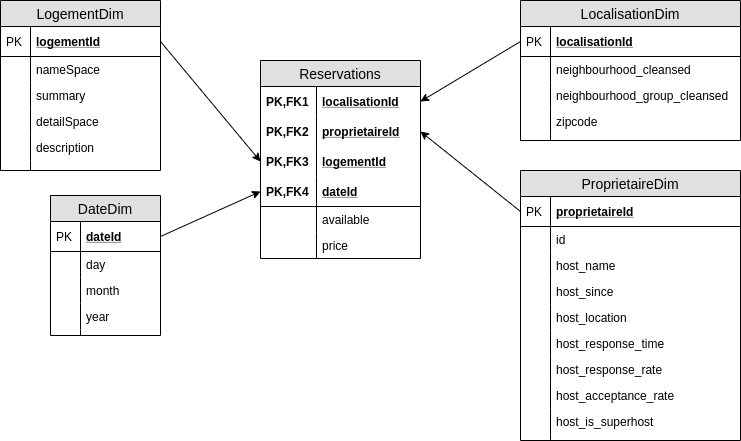
\includegraphics[width=0.9\linewidth]{./schema_entrepot.png}
   \end{center}
\end{figure}

\section{Opérations sur l'entrepôt}
\subsection{Requêtes :}
\tab Voici les requêtes que nous avons réalisés sur notre entrepôt --- elles peuvent être exécutées via le fichier \Verb|projet.sql| en annexe du rapport :
\begin{itemize}[label=\textbullet]
   \item Requête n$^\circ$1 :
   Permet d'obtenir le nombre de logements différents par années et au totale.
   \begin{lstlisting}
   SELECT year, count(DISTINCT logementId)
   FROM DateDim NATURAL JOIN LogementDim NATURAL JOIN Reservations
   GROUP BY year WITH ROLLUP;
   \end{lstlisting}
   \item Requête n$^\circ$2 :
   Permet d'obtenir le nombre de logement par code postal, par an et totale.
   \begin{lstlisting}
   SELECT zipcode, year, count(DISTINCT logementId)
   FROM DateDim NATURAL JOIN LocalisationDim NATURAL JOIN LogementDim
      NATURAL JOIN Reservations
   GROUP BY zipcode, year WITH ROLLUP;
   \end{lstlisting}
   \item Requête n$^\circ$3 :
   Permet d'obtenir le prix que peut gagner chaque région, par mois, par années et au totale.
   \begin{lstlisting}
   SELECT zipcode, year, month, SUM(price)
   FROM DateDim NATURAL JOIN LocalisationDim NATURAL JOIN Reservations
   WHERE available = 't'
   GROUP BY zipcode, year, month WITH ROLLUP;
   \end{lstlisting}
   \item Requête n$^\circ$4 :
   Permet d'obtenir le prix moyen par an, par région et au total.
   \begin{lstlisting}
   SELECT zipcode, year, avg(price)
   FROM DateDim NATURAL JOIN LocalisationDim NATURAL JOIN Reservations
   WHERE price IS NOT NULL
   GROUP BY zipcode, year WITH ROLLUP;
   \end{lstlisting}
   \item Requête n$^\circ$5 :
   Permet d'obtenir le rang des 20 personnes qui gagne le plus.
   \begin{lstlisting}
   SET @curRank := 0;
   SELECT *, @curRank := @curRank + 1 AS rank FROM (
      SELECT proprietaireId, host_name, year, SUM(price)
      FROM DateDim NATURAL JOIN LocalisationDim NATURAL JOIN ProprietaireDim
         NATURAL JOIN Reservations
      GROUP BY proprietaireId, year
      ORDER BY SUM(price) DESC
   ) AS t LIMIT 20;
   \end{lstlisting}
   \item Requête n$^\circ$6 :
   Permet d'afficher le nombre de proprietaire par région et au total.
   \begin{lstlisting}
   SELECT zipcode, count(DISTINCT proprietaireId)
   FROM LocalisationDim NATURAL JOIN ProprietaireDim NATURAL JOIN Reservations
   GROUP BY zipcode WITH ROLLUP;
   \end{lstlisting}
   \item Requête n$^\circ$7 :
   Permet d'obtenir le nombre de fois qu'un propriétaire a obtenu le titre de superhost par région et au total.
   \begin{lstlisting}
   SELECT zipcode, count(proprietaireId)
   FROM LocalisationDim NATURAL JOIN ProprietaireDim NATURAL JOIN Reservations
   WHERE host_is_superhost = 't'
   GROUP BY zipcode WITH ROLLUP;
   \end{lstlisting}
   \item Requête n$^\circ$8 :
   Permet d'afficher le nombre de response\_rate de chaque hote, et le nombre total.
   \begin{lstlisting}
   SELECT host_name, host_response_rate, count(*)
   FROM ProprietaireDim NATURAL JOIN Reservations
   WHERE host_response_rate IS NOT NULL
   GROUP BY host_response_rate, host_name WITH ROLLUP;
   \end{lstlisting}
\end{itemize}

\subsection{Résultats :}
\tab Voici les résultats de nos requêtes précédentes --- pour obtenir la totalité de celles-ci, vous pouvez aller voir dans le fichier annexe \Verb|result.txt| :
\lstset{basicstyle=\tiny}
\begin{itemize}[label=\textbullet]
   \item Résultats n$^\circ$1 :
   \begin{lstlisting}
   +------+----------------------------+
   | year | count(DISTINCT logementId) |
   +------+----------------------------+
   | 2016 |                        270 |
   | 2017 |                        269 |
   | NULL |                        270 |
   +------+----------------------------+
   \end{lstlisting}
   \item Résultats n$^\circ$2 :
   \begin{lstlisting}
   +---------+------+----------------------------+
   | zipcode | year | count(DISTINCT logementId) |
   +---------+------+----------------------------+
   |   98107 | 2016 |                        128 |
   |   98107 | 2017 |                        128 |
   |   98107 | NULL |                        128 |
   |   98109 | 2016 |                         74 |
   |   98109 | 2017 |                         73 |
   |   98109 | NULL |                         74 |
   |   98117 | 2016 |                          4 |
   |   98117 | 2017 |                          4 |
   |   98117 | NULL |                          4 |
   |   98119 | 2016 |                         64 |
   |   98119 | 2017 |                         64 |
   |   98119 | NULL |                         64 |
   |    NULL | NULL |                        270 |
   +---------+------+----------------------------+
   \end{lstlisting}
   \pagebreak
   \item Résultats n$^\circ$3 :
   \begin{lstlisting}
   +---------+------+-------+------------+
   | zipcode | year | month | SUM(price) |
   +---------+------+-------+------------+
   |   98107 | 2016 |     1 |     198981 |
   |   98107 | 2016 |     2 |     255808 |
   |   98107 | 2016 |     3 |     314406 |
   |   98107 | 2016 |     4 |     299849 |
   |   98107 | 2016 |     5 |     319755 |
   |   98107 | 2016 |     6 |     374994 |
   |   98107 | 2016 |     7 |     331889 |
   |   98107 | 2016 |     8 |     354556 |
   |   98107 | 2016 |     9 |     328862 |
   |   98107 | 2016 |    10 |     343146 |
   |   98107 | 2016 |    11 |     334926 |
   |   98107 | 2016 |    12 |     368250 |
   |   98107 | 2016 |  NULL |    3825422 |
   |   98107 | 2017 |     1 |      23901 |
   |   98107 | 2017 |  NULL |      23901 |
   |   98107 | NULL |  NULL |    3849323 |
   |   98109 | 2016 |     1 |     209538 |
   |   98109 | 2016 |     2 |     249775 |

   etc...
   \end{lstlisting}
   \item Résultats n$^\circ$4 :
   \begin{lstlisting}
   +---------+------+--------------------+
   | zipcode | year | AVG(price)         |
   +---------+------+--------------------+
   |   98107 | 2016 | 125.09964354622453 |
   |   98107 | 2017 | 127.13297872340425 |
   |   98107 | NULL | 125.11206812493906 |
   |   98109 | 2016 | 169.36099685458504 |
   |   98109 | 2017 | 163.74257425742573 |
   |   98109 | NULL | 169.32688029820238 |
   |   98117 | 2016 |  109.7921568627451 |
   |   98117 | 2017 |              147.5 |
   |   98117 | NULL | 110.23062015503876 |
   |   98119 | 2016 |  199.1352493660186 |
   |   98119 | 2017 | 213.37037037037038 |
   |   98119 | NULL |    199.23451927423 |
   |    NULL | NULL | 154.69553491159724 |
   +---------+------+--------------------+
   \end{lstlisting}
   \item Résultats n$^\circ$5 :
   \begin{lstlisting}
   +----------------+--------------------+------+------------+------+
   | proprietaireId | host_name          | year | SUM(price) | rank |
   +----------------+--------------------+------+------------+------+
   |       32713558 | Kary               | 2016 |     249900 |    1 |
   |       22372266 | Sarah              | 2016 |     218018 |    2 |
   |         919364 | Jeff               | 2016 |     217800 |    3 |
   |       16708587 | Jill               | 2016 |     205848 |    4 |
   |       28770702 | Mercy              | 2016 |     186119 |    5 |
   |       24049136 | Jeff               | 2016 |     178642 |    6 |
   |         430709 | Sea To Sky Rentals | 2016 |     173015 |    7 |
   |        1452570 | Emily              | 2016 |     168000 |    8 |
   |        3792761 | Kimberly           | 2016 |     165790 |    9 |
   |        6407320 | Varun              | 2016 |     163460 |   10 |
   |        5177328 | Andrea             | 2016 |     163354 |   11 |
   |       23669617 | Irmela             | 2016 |     145200 |   12 |
   |       24633415 | David              | 2016 |     145183 |   13 |
   |        2231298 | Chris              | 2016 |     136647 |   14 |
   |       33147763 | Tracy              | 2016 |     126000 |   15 |
   |       12867960 | Maureen            | 2016 |     122337 |   16 |
   |       19993125 | Steven             | 2016 |     122020 |   17 |
   |        6097842 | Brittain           | 2016 |     118615 |   18 |
   |       33225983 | Jean               | 2016 |     117047 |   19 |
   |       31148752 | Bo                 | 2016 |     108658 |   20 |
   +----------------+--------------------+------+------------+------+
   \end{lstlisting}
   \item Résultats n$^\circ$6 :
   \begin{lstlisting}
   +---------+--------------------------------+
   | zipcode | count(DISTINCT proprietaireId) |
   +---------+--------------------------------+
   |   98107 |                            110 |
   |   98109 |                             67 |
   |   98117 |                              4 |
   |   98119 |                             56 |
   |    NULL |                            233 |
   +---------+--------------------------------+
   \end{lstlisting}
   \item Résultats n$^\circ$7 :
   \begin{lstlisting}
   +---------+-----------------------+
   | zipcode | count(proprietaireId) |
   +---------+-----------------------+
   |   98107 |                 13870 |
   |   98109 |                  6014 |
   |   98117 |                   365 |
   |   98119 |                  4745 |
   |    NULL |                 24994 |
   +---------+-----------------------+
   \end{lstlisting}
   \pagebreak
   \item Résultats n$^\circ$8 :
   \begin{lstlisting}
   +---------------------+--------------------+----------+
   | host_name           | host_response_rate | count(*) |
   +---------------------+--------------------+----------+
   | Alan                | 100%               |      365 |
   | Alan & Katence      | 100%               |      365 |
   | Alex                | 100%               |      730 |
   | Alexis              | 100%               |      365 |
   | Alianna             | 100%               |      365 |
   | Aman                | 100%               |      365 |
   | Amber               | 100%               |      365 |
   | Amelia & Foxy       | 100%               |      365 |
   | Andrea              | 100%               |      730 |
   | Andrew              | 100%               |      365 |
   | Anisa               | 100%               |      365 |
   | Annie               | 100%               |      730 |
   | Audrey              | 100%               |      365 |
   | Barbara             | 100%               |      730 |
   | Barrie              | 100%               |      365 |
   | Bill                | 100%               |      365 |
   | Bob                 | 100%               |      730 |
   | Brad & Liz          | 100%               |      730 |
   | Brian               | 100%               |      730 |
   | Brittain            | 100%               |      730 |

   etc...
   \end{lstlisting}
\end{itemize}

\section{Conclusion}
\tab Le fait de devoir concevoir un entrepôt n'est pas chose si facile. En effet, il d'abord réussir à trouver le bon jeu de données avec les bonnes licences. Ensuite, il faut créer notre entrepôt avec le schéma en étoile. Arrive la tâche la plus éprouvante et la moins intéressante qui est le nettoyage des données. Cela est extrêment chronophage car en général, les données brutes ne sont jamais homogène. Et pour finir arrive l'étape des requêtes.\\
\tab Au cours de ce projet, nous nous sommes heurté à plusieurs problèmes. Nous avons d'abord changé 3 fois de dataset. En effet, les deux premiers n'étaient pas si intéressant après consultation, mais aussi beaucoup de données manquantes. Ensuite, le nettoyage de données posa problème. Le fait que \url{https://livesql.oracle.com/} n'acceptait pas les caractères non ASCII n'était pas facile à repérer. En effet, quand nous essayions d'insérer nos tables dedans, lorsqu'une erreur apparaissait, nous n'avions aucun log de nos erreurs. Il était seulement affiché erreur en gros. Pour finir, \url{https://livesql.oracle.com/} posant énormement de problèmes, car n'acceptait que des fichiers pesant moins de 1Mb, nous avons décidé de passer sous MySQL, limitant nos possibilités de requêtes.
\end{document}
